% Generated by zju-lab-report.
% Edit the Markdown source and metadata, not this LaTeX file.
\documentclass[UTF8,a4paper,12pt]{ctexart}

\usepackage[left=2.6cm,right=2.6cm,top=2.8cm,bottom=2.8cm]{geometry}
\usepackage{graphicx}
\usepackage{float}
\usepackage{booktabs}
\usepackage{array}
\usepackage{amsmath,amssymb}
\usepackage{caption}
\usepackage{subcaption}
\usepackage{fancyhdr}
\usepackage{setspace}
\usepackage{titlesec}
\usepackage{tocloft}
\usepackage[table]{xcolor}
\usepackage{tabularx}
\usepackage{makecell}
\usepackage{enumitem}
\usepackage{hyperref}
\usepackage{needspace}

\usepackage{color}
\usepackage{fancyvrb}
\newcommand{\VerbBar}{|}
\newcommand{\VERB}{\Verb[commandchars=\\\{\}]}
\DefineVerbatimEnvironment{Highlighting}{Verbatim}{commandchars=\\\{\}}
% Add ',fontsize=\small' for more characters per line
\newenvironment{Shaded}{}{}
\newcommand{\AlertTok}[1]{\textcolor[rgb]{1.00,0.00,0.00}{\textbf{#1}}}
\newcommand{\AnnotationTok}[1]{\textcolor[rgb]{0.38,0.63,0.69}{\textbf{\textit{#1}}}}
\newcommand{\AttributeTok}[1]{\textcolor[rgb]{0.49,0.56,0.16}{#1}}
\newcommand{\BaseNTok}[1]{\textcolor[rgb]{0.25,0.63,0.44}{#1}}
\newcommand{\BuiltInTok}[1]{\textcolor[rgb]{0.00,0.50,0.00}{#1}}
\newcommand{\CharTok}[1]{\textcolor[rgb]{0.25,0.44,0.63}{#1}}
\newcommand{\CommentTok}[1]{\textcolor[rgb]{0.38,0.63,0.69}{\textit{#1}}}
\newcommand{\CommentVarTok}[1]{\textcolor[rgb]{0.38,0.63,0.69}{\textbf{\textit{#1}}}}
\newcommand{\ConstantTok}[1]{\textcolor[rgb]{0.53,0.00,0.00}{#1}}
\newcommand{\ControlFlowTok}[1]{\textcolor[rgb]{0.00,0.44,0.13}{\textbf{#1}}}
\newcommand{\DataTypeTok}[1]{\textcolor[rgb]{0.56,0.13,0.00}{#1}}
\newcommand{\DecValTok}[1]{\textcolor[rgb]{0.25,0.63,0.44}{#1}}
\newcommand{\DocumentationTok}[1]{\textcolor[rgb]{0.73,0.13,0.13}{\textit{#1}}}
\newcommand{\ErrorTok}[1]{\textcolor[rgb]{1.00,0.00,0.00}{\textbf{#1}}}
\newcommand{\ExtensionTok}[1]{#1}
\newcommand{\FloatTok}[1]{\textcolor[rgb]{0.25,0.63,0.44}{#1}}
\newcommand{\FunctionTok}[1]{\textcolor[rgb]{0.02,0.16,0.49}{#1}}
\newcommand{\ImportTok}[1]{\textcolor[rgb]{0.00,0.50,0.00}{\textbf{#1}}}
\newcommand{\InformationTok}[1]{\textcolor[rgb]{0.38,0.63,0.69}{\textbf{\textit{#1}}}}
\newcommand{\KeywordTok}[1]{\textcolor[rgb]{0.00,0.44,0.13}{\textbf{#1}}}
\newcommand{\NormalTok}[1]{#1}
\newcommand{\OperatorTok}[1]{\textcolor[rgb]{0.40,0.40,0.40}{#1}}
\newcommand{\OtherTok}[1]{\textcolor[rgb]{0.00,0.44,0.13}{#1}}
\newcommand{\PreprocessorTok}[1]{\textcolor[rgb]{0.74,0.48,0.00}{#1}}
\newcommand{\RegionMarkerTok}[1]{#1}
\newcommand{\SpecialCharTok}[1]{\textcolor[rgb]{0.25,0.44,0.63}{#1}}
\newcommand{\SpecialStringTok}[1]{\textcolor[rgb]{0.73,0.40,0.53}{#1}}
\newcommand{\StringTok}[1]{\textcolor[rgb]{0.25,0.44,0.63}{#1}}
\newcommand{\VariableTok}[1]{\textcolor[rgb]{0.10,0.09,0.49}{#1}}
\newcommand{\VerbatimStringTok}[1]{\textcolor[rgb]{0.25,0.44,0.63}{#1}}
\newcommand{\WarningTok}[1]{\textcolor[rgb]{0.38,0.63,0.69}{\textbf{\textit{#1}}}}

\usepackage{calc}
\usepackage{longtable}
\usepackage{xurl}
\usepackage[most]{tcolorbox}
\usepackage{fvextra}
\graphicspath{{./}{../}}
\makeatletter\def\fps@figure{H}\makeatother
\newcounter{none}
\Urlmuskip=0mu plus 2mu
\definecolor{zjucodebg}{HTML}{F7F9FC}
\definecolor{zjucodeframe}{HTML}{D7E1F0}
\definecolor{zjucodebar}{HTML}{3B82F6}
\RecustomVerbatimEnvironment{Highlighting}{Verbatim}{commandchars=\\\{\},fontsize=\small,breaklines=true,breakanywhere=true}
\renewenvironment{Shaded}{\vspace{0.35em}\begin{tcolorbox}[enhanced,breakable,colback=zjucodebg,colframe=zjucodeframe,boxrule=0.45pt,leftrule=2.2pt,arc=1.6mm,left=1.8mm,right=1.8mm,top=1.2mm,bottom=1.2mm]}{\end{tcolorbox}\vspace{0.25em}}
\providecommand{\tightlist}{\setlength{\itemsep}{0pt}\setlength{\parskip}{0pt}}
\newsavebox{\pandocboundedbox}
\providecommand{\pandocbounded}[1]{#1}
\renewcommand{\pandocbounded}[1]{\sbox{\pandocboundedbox}{#1}\ifdim\wd\pandocboundedbox>\linewidth\resizebox{\linewidth}{!}{#1}\else#1\fi}

\hypersetup{
  colorlinks=true,
  linkcolor=black,
  urlcolor=blue,
  citecolor=black
}

\setstretch{1.3}
\setlength{\parindent}{2em}
\setlength{\parskip}{0.3em}
\captionsetup{font=small,labelfont=bf}
\setlist[itemize]{leftmargin=2.5em}
\setlist[enumerate]{leftmargin=2.8em}
\newcolumntype{Y}{>{\raggedright\arraybackslash}X}
\newcolumntype{Z}{>{\centering\arraybackslash}X}
\definecolor{zjutablehead}{gray}{0.88}
\definecolor{zjutablefirst}{gray}{0.92}

\titleformat{\section}{\heiti\zihao{3}}{\thesection}{0.8em}{}
\titleformat{\subsection}{\heiti\zihao{-3}}{\thesubsection}{0.8em}{}
\titleformat{\subsubsection}{\heiti\zihao{4}}{\thesubsubsection}{0.8em}{}

\renewcommand\contentsname{目录}
\renewcommand\cftsecleader{\cftdotfill{\cftdotsep}}
\renewcommand\cftsubsecleader{\cftdotfill{\cftdotsep}}

\pagestyle{fancy}
\fancyhf{}
\fancyhead[L]{自然语言处理导论\ 实验报告}
\fancyhead[R]{黄晗\quad 刘泽晖\quad 王子朔\quad 赵一帆\quad 叶顺凡}
\cfoot{\thepage}
\renewcommand{\headrulewidth}{0.4pt}

\setcounter{secnumdepth}{3}
\setcounter{tocdepth}{2}

\newcommand{\reporttitle}{基于 GRPO 与可验证奖励的 24 点游戏求解}
\newcommand{\reportcourse}{自然语言处理导论}
\newcommand{\reporttype}{实验报告}
\newcommand{\reportauthor}{黄晗\quad 刘泽晖\quad 王子朔\quad 赵一帆\quad 叶顺凡}
\newcommand{\reportcollege}{计算机科学与技术学院}
\newcommand{\reportmajor}{计算机科学与技术}
\newcommand{\reportadvisor}{汤斯亮}
\newcommand{\reportdate}{2026 年 6 月 14 日}
\newcommand{\reportlogopath}{/Users/hanhuang/.codex/skills/zju-lab-report/assets/zju-logo.png}
\newcommand{\infovalue}[1]{\underline{\makebox[8.6cm][c]{#1}}}

\begin{document}

\begin{titlepage}
    \thispagestyle{empty}
    \centering

    \vspace*{1.2cm}
        \includegraphics[width=0.72\textwidth]{\reportlogopath}
    
    \vspace{3.0cm}
    {\heiti\zihao{2} \reportcourse\quad \reporttype\par}

    \vspace{1.8cm}
    {\heiti\zihao{3}
    \begin{minipage}{0.86\textwidth}
        \centering
        \reporttitle\par
        \vspace{0.25em}
        \hrule height 0.4pt
    \end{minipage}
    \par}

    \vfill

    {\zihao{4}
    \renewcommand{\arraystretch}{1.95}
    \begin{tabular}{>{\heiti}p{3.0cm}<{\centering} p{9.0cm}<{\centering}}
        成员 & \infovalue{\reportauthor} \\
        学院 & \infovalue{\reportcollege} \\
        专业 & \infovalue{\reportmajor} \\
        指导老师 & \infovalue{\reportadvisor} \\
    \end{tabular}
    }

    \vspace{2.0cm}
    {\zihao{4} \reportdate\par}
\end{titlepage}

\clearpage
\tableofcontents
\clearpage

\begin{center}
    {\heiti\zihao{3} \reporttitle\par}
    \vspace{0.8em}
    {\heiti\zihao{-2} 摘\ 要\par}
\end{center}

本次实验我们面向 24 点游戏构建了一个可验证奖励强化学习（RLVR）实验系统。给定 4 个 1-13 之间的整数，模型需要按照 R1 风格输出一个只使用四则运算和括号的表达式，并且每个输入数字恰好使用一次、结果等于 24。实验以 Qwen2.5-1.5B-Instruct 为主线，采用 SFT warm-up 建立基本表达式生成能力，再使用 GRPO 进行可验证奖励强化学习。

最终结果显示，SFT+GRPO + verifier best-of-16 在 Official OOD split 上达到 65.5\%，在 Tree of Thoughts hard split 900-1000 上达到 49.0\%，不可解样本幻觉率为 0.0\%。除主任务外，项目还将验证器、prompt 与 reward 扩展为 target-aware 形式，在 Countdown 任意目标数任务上完成加分项验证。

\clearpage

\section{引言与贡献}\label{ux5f15ux8a00ux4e0eux8d21ux732e}

24 点游戏是一个典型的小规模组合推理任务。它既要求模型理解自然语言 prompt，又要求模型完成离散搜索、算术计算和格式约束。更重要的是，答案是否正确可以由程序严格验证，因此它非常适合作为 RLVR 场景：不需要人工偏好标注，也不需要训练额外奖励模型。

相关工作为本项目提供了三条技术脉络：DeepSeekMath 提出 GRPO，以组内相对奖励降低策略优化成本{[}1{]}；DeepSeek-R1 与 Logic-RL 展示了规则奖励强化学习对推理能力的激励作用{[}2,7{]}；Tree of Thoughts 在 24 点任务上验证了多路径搜索的价值{[}5{]}，TinyZero 则将类似思想用于 Countdown 等可验证算术任务{[}6{]}。本项目在此基础上采用更轻量的 SFT+GRPO 与符号验证器组合，并参考 TRL 和 Open-R1 的开放训练工具链{[}9-10{]}。

本次实验我们的主要工作和亮点如下：

\begin{enumerate}
\def\labelenumi{\arabic{enumi}.}
\tightlist
\item
  构建了 \texttt{Qwen2.5-1.5B-Instruct} 的完整训练闭环：base evaluation、SFT warm-up、SFT 后 GRPO continuation。
\item
  将 24 点任务统一建模为 \texttt{(numbers,\ target)\ -\textgreater{}\ expression}，使同一套 verifier/reward 可迁移到 Countdown 任意目标数任务。
\item
  显式引入不可解样本评估，将模型``会不会解题''和``会不会拒绝乱编''同时纳入评价。
\item
  使用 verifier-based test-time compute，将模型输出建模为候选表达式生成，并用程序验证器筛选正确解。
\item
  对结果进行错误类型、hard split 难度和 GRPO 超参稳定性分析，避免只报告单一准确率。
\end{enumerate}

\section{任务定义与挑战分析}\label{ux4efbux52a1ux5b9aux4e49ux4e0eux6311ux6218ux5206ux6790}

\subsection{任务定义}\label{ux4efbux52a1ux5b9aux4e49}

24 点主任务输入为 4 个整数：

\begin{Shaded}
\begin{Highlighting}[]
\NormalTok{numbers = [a, b, c, d],  a,b,c,d in \{1, ..., 13\}}
\NormalTok{target = 24}
\end{Highlighting}
\end{Shaded}

模型输出必须满足：

\begin{Shaded}
\begin{Highlighting}[]
\NormalTok{\textless{}think\textgreater{}reasoning process\textless{}/think\textgreater{}}
\NormalTok{\textless{}answer\textgreater{}expression\textless{}/answer\textgreater{}}
\end{Highlighting}
\end{Shaded}

其中 \texttt{expression} 只能包含输入数字、四则运算符 \texttt{+\ -\ *\ /} 与括号。验证器检查三类约束：

\begin{enumerate}
\def\labelenumi{\arabic{enumi}.}
\tightlist
\item
  数字使用约束：每个输入数字必须且只能使用一次。
\item
  语法安全约束：表达式只允许四则运算和括号。
\item
  目标值约束：表达式计算结果与 target 的误差不超过 \texttt{1e-6}。
\end{enumerate}

对于不可解输入，模型应输出 \texttt{NO\_SOLUTION}，而不是强行编造表达式。

\subsection{主要挑战}\label{ux4e3bux8981ux6311ux6218}

\textbf{组合搜索空间大。} 24 点求解涉及数字排列、运算符选择和括号结构组合。模型需要隐式完成离散搜索，而不是简单记忆答案。

\textbf{奖励稀疏。} 只有完整表达式通过验证器时才获得准确率奖励，部分正确的中间步骤通常无法直接得分。

\textbf{格式与语义双重约束。} 模型既要遵守 DeepSeek-R1 类 \texttt{\textless{}think\textgreater{}/\textless{}answer\textgreater{}} 输出模板{[}2{]}，又要保证 \texttt{\textless{}answer\textgreater{}} 内表达式真实可执行、可验证。

\textbf{不可解样本存在幻觉风险。} 大语言模型倾向于生成看似合理的答案。对不可解样本，如果没有单独建模，模型可能始终输出一个错误表达式。

\textbf{强化学习训练不稳定。} GRPO 可以提升候选池质量，但也可能扰动 SFT 后的拒答行为，导致 greedy 下 hallucination 上升。

\section{问题建模与创新设计}\label{ux95eeux9898ux5efaux6a21ux4e0eux521bux65b0ux8bbeux8ba1}

\begin{figure}
\centering
\pandocbounded{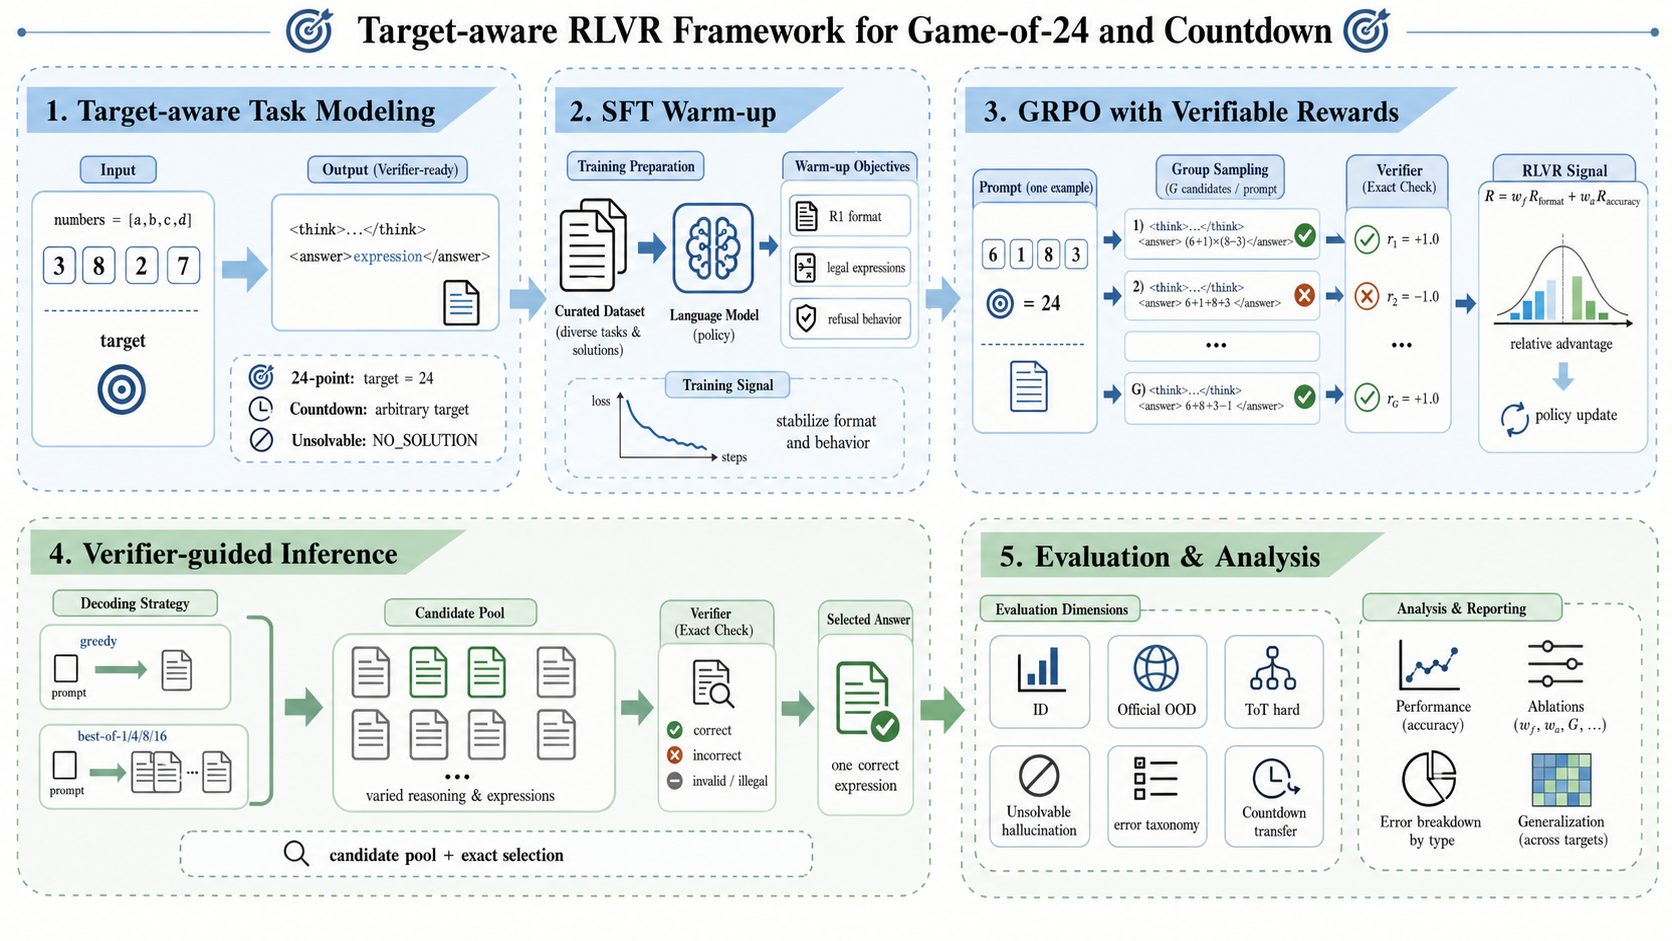
\includegraphics[keepaspectratio,alt={方法总图}]{figures/method_overview.png}}
\caption{方法总图}
\end{figure}

\subsection{Target-aware 统一建模}\label{target-aware-ux7edfux4e00ux5efaux6a21}

我们没有将验证器写死为 24，而是将任务统一表示为：

\begin{Shaded}
\begin{Highlighting}[]
\NormalTok{(numbers, target) {-}\textgreater{} expression}
\end{Highlighting}
\end{Shaded}

24 点是 \texttt{target=24} 的特例。Countdown 任务则使用每条样本自己的 target，因此 prompt、reward、verifier 和 evaluation 均可复用。这使系统从固定 24 点求解器扩展为通用的小规模算术目标构造器。

\subsection{Verifier-based RLVR}\label{verifier-based-rlvr}

奖励不依赖人工标注或奖励模型，而由程序验证器直接给出。验证器基于 AST 安全解析表达式，过滤非法语法、非法数字使用和错误结果。这样的奖励完全可复现，也避免了自然语言奖励模型在算术任务上的不稳定判断。

\subsection{不可解样本的 Hallucination 建模}\label{ux4e0dux53efux89e3ux6837ux672cux7684-hallucination-ux5efaux6a21}

我们将不可解样本作为独立 split。若模型在不可解题中输出错误表达式，则记为 hallucination；若输出 \texttt{NO\_SOLUTION} 或等价拒答，则视为正确拒答。该设计把任务从``只求解可解题''扩展为``求解与可解性判断''的联合问题。

\subsection{Verifier-based Test-time Compute}\label{verifier-based-test-time-compute}

单次 greedy 输出无法充分反映模型候选池中的潜在能力。为此，我们在测试时采样多个候选，并用验证器选择第一个正确表达式。该过程等价于：

\begin{Shaded}
\begin{Highlighting}[]
\NormalTok{language model {-}\textgreater{} candidate pool {-}\textgreater{} verifier selection}
\end{Highlighting}
\end{Shaded}

这与 Tree of Thoughts{[}5{]} 和 TinyZero{[}6{]} 的思想一致，但实现更轻量：不需要人工打分，也不需要额外搜索模型。

\section{方法}\label{ux65b9ux6cd5}

\subsection{Prompt 与输出格式}\label{prompt-ux4e0eux8f93ux51faux683cux5f0f}

训练和评估均使用 R1 风格模板：

\begin{Shaded}
\begin{Highlighting}[]
\NormalTok{\textless{}think\textgreater{}}
\NormalTok{brief reasoning process}
\NormalTok{\textless{}/think\textgreater{}}
\NormalTok{\textless{}answer\textgreater{}}
\NormalTok{(1+2+3)*4}
\NormalTok{\textless{}/answer\textgreater{}}
\end{Highlighting}
\end{Shaded}

评估时只验证 \texttt{\textless{}answer\textgreater{}} 中的表达式。这样既保留 reasoning 格式，又避免将自然语言推理文本纳入算术验证。

\subsection{安全表达式验证器}\label{ux5b89ux5168ux8868ux8fbeux5f0fux9a8cux8bc1ux5668}

验证器执行以下步骤：

\begin{enumerate}
\def\labelenumi{\arabic{enumi}.}
\tightlist
\item
  从 completion 中抽取 \texttt{\textless{}answer\textgreater{}}。
\item
  若答案为 \texttt{NO\_SOLUTION}，进入不可解样本拒答判断。
\item
  使用 AST 解析表达式，拒绝函数调用、变量、列表等非四则运算语法。
\item
  统计表达式中出现的数字，与输入 multiset 精确匹配。
\item
  计算表达式值，判断是否满足 \texttt{abs(value\ -\ target)\ \textless{}=\ 1e-6}。
\end{enumerate}

\subsection{奖励函数}\label{ux5956ux52b1ux51fdux6570}

GRPO 训练使用格式奖励和准确率奖励的加权组合：

\begin{Shaded}
\begin{Highlighting}[]
\NormalTok{R = w\_f R\_format + w\_a R\_accuracy}
\end{Highlighting}
\end{Shaded}

\begin{figure}
\centering
\pandocbounded{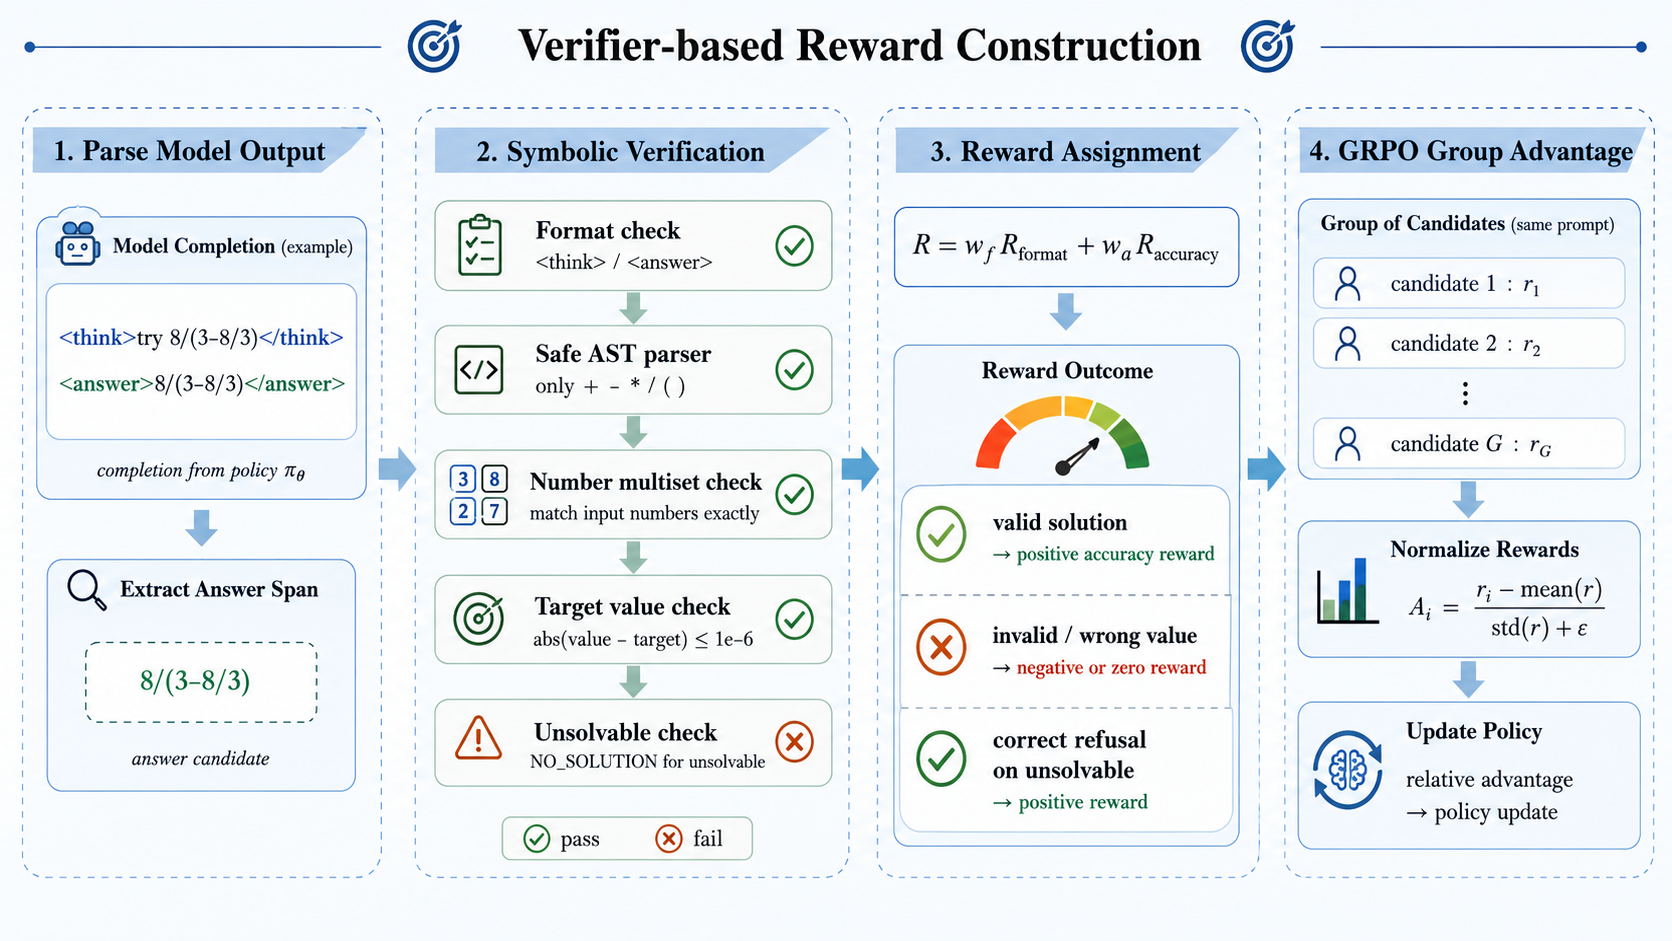
\includegraphics[keepaspectratio,alt={Verifier/reward 构造}]{figures/verifier_reward.png}}
\caption{Verifier/reward 构造}
\end{figure}

其中 \texttt{R\_format} 检查 \texttt{\textless{}think\textgreater{}} 与 \texttt{\textless{}answer\textgreater{}} 标签是否完整，\texttt{R\_accuracy} 检查答案是否通过验证器。对于不可解样本，正确拒答获得正向奖励，乱编表达式受到惩罚。

\subsection{SFT Warm-up}\label{sft-warm-up}

直接对基础模型做 GRPO 容易学到格式捷径，例如只输出固定标签或固定数字。为缓解稀疏奖励问题，我们先使用可验证表达式进行 SFT warm-up，使模型具备：

\begin{enumerate}
\def\labelenumi{\arabic{enumi}.}
\tightlist
\item
  稳定输出 R1 格式的能力；
\item
  生成合法表达式的基本能力；
\item
  在不可解样本上输出拒答的能力。
\end{enumerate}

SFT 后再进行 GRPO，强化学习主要用于改善候选表达式质量，而不是从零学习格式。

\subsection{GRPO 训练}\label{grpo-ux8badux7ec3}

GRPO 对同一个 prompt 采样一组候选，根据组内相对奖励计算优势{[}1{]}。设同组奖励为 \texttt{r\_1,\ ...,\ r\_G}，则第 \texttt{i} 个候选的优势为：

\begin{Shaded}
\begin{Highlighting}[]
\NormalTok{A\_i = (r\_i {-} mean(r)) / (std(r) + epsilon)}
\end{Highlighting}
\end{Shaded}

训练流程如下：

\begin{Shaded}
\begin{Highlighting}[]
\ControlFlowTok{for}\NormalTok{ prompt }\KeywordTok{in}\NormalTok{ training\_prompts:}
\NormalTok{    candidates }\OperatorTok{=}\NormalTok{ sample(model, prompt, G)}
\NormalTok{    rewards }\OperatorTok{=}\NormalTok{ [verifier\_reward(c) }\ControlFlowTok{for}\NormalTok{ c }\KeywordTok{in}\NormalTok{ candidates]}
\NormalTok{    advantages }\OperatorTok{=}\NormalTok{ normalize\_within\_group(rewards)}
\NormalTok{    update\_policy\_with\_GRPO(candidates, advantages)}
\end{Highlighting}
\end{Shaded}

本次实验主线使用 \texttt{GRPO\_SAMPLES=300}、\texttt{GRPO\_GENERATIONS=8}，并补充低学习率对照以分析训练稳定性。

\subsection{Best-of-N Verifier 解码}\label{best-of-n-verifier-ux89e3ux7801}

评估阶段的 best-of-N 不改变模型参数，只增加测试时采样候选数：

\begin{Shaded}
\begin{Highlighting}[]
\ControlFlowTok{for}\NormalTok{ problem }\KeywordTok{in}\NormalTok{ test\_set:}
\NormalTok{    candidates }\OperatorTok{=}\NormalTok{ sample(model, problem, N)}
    \ControlFlowTok{for}\NormalTok{ candidate }\KeywordTok{in}\NormalTok{ candidates:}
        \ControlFlowTok{if}\NormalTok{ verifier(candidate) }\OperatorTok{==}\NormalTok{ correct:}
            \ControlFlowTok{return}\NormalTok{ candidate}
    \ControlFlowTok{if}\NormalTok{ problem }\KeywordTok{is}\NormalTok{ unsolvable }\KeywordTok{and} \BuiltInTok{any}\NormalTok{ candidate }\KeywordTok{is}\NormalTok{ NO\_SOLUTION:}
        \ControlFlowTok{return}\NormalTok{ NO\_SOLUTION}
    \ControlFlowTok{return}\NormalTok{ failed}
\end{Highlighting}
\end{Shaded}

\begin{figure}
\centering
\pandocbounded{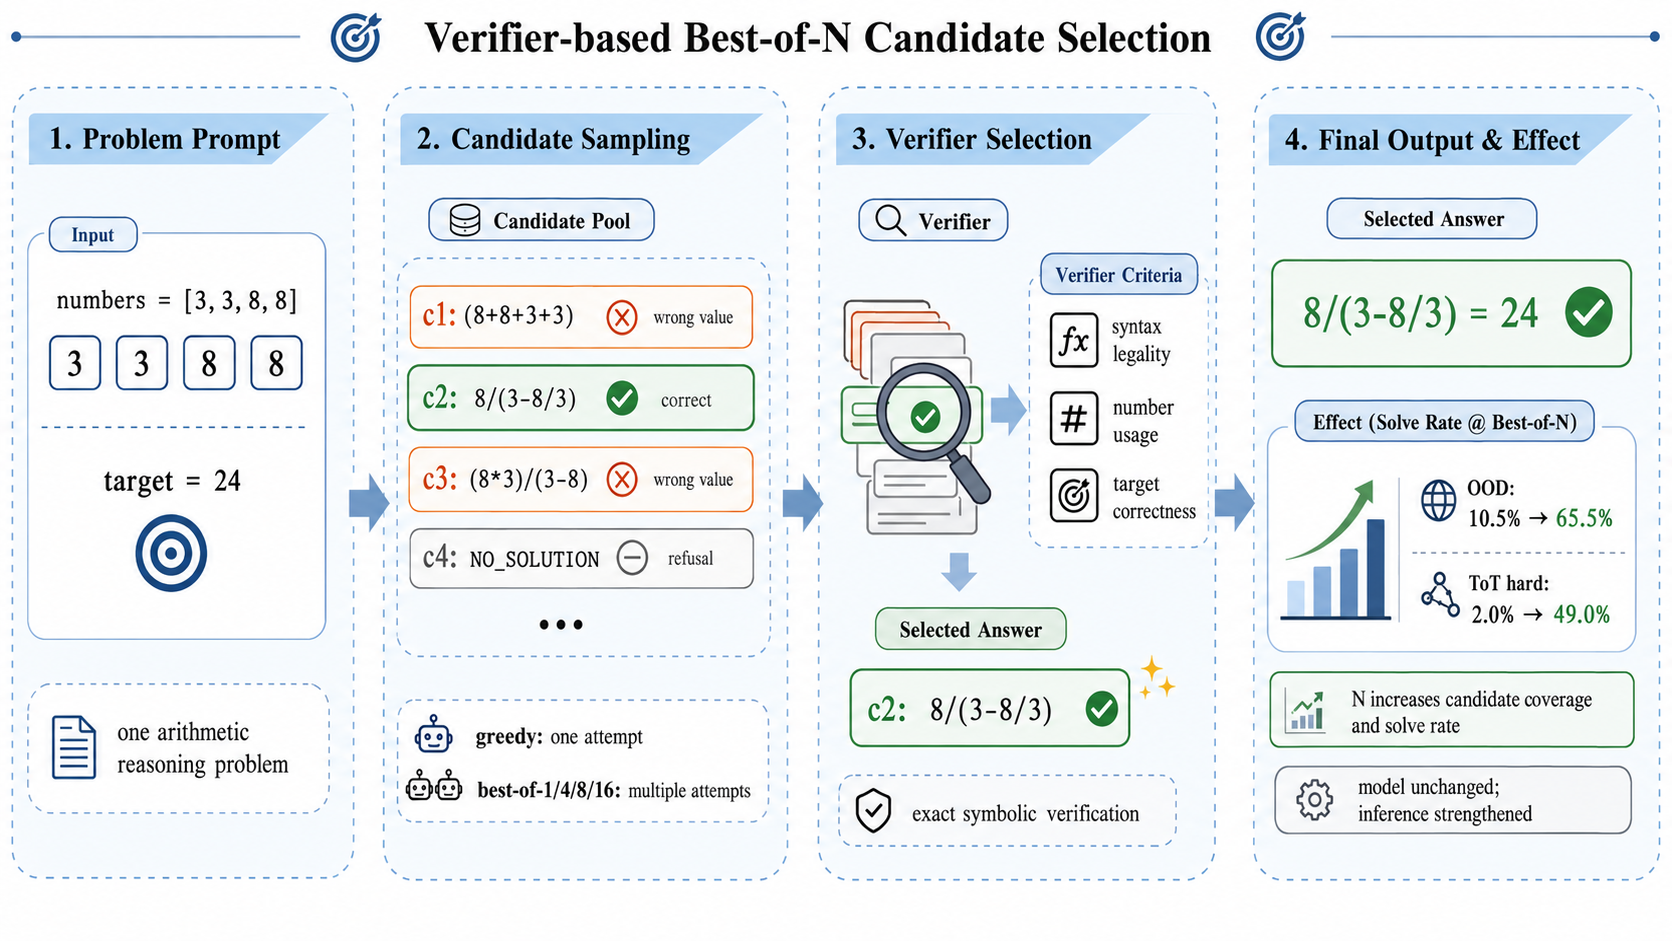
\includegraphics[keepaspectratio,alt={Best-of-N 机制图}]{figures/bestof_mechanism.png}}
\caption{Best-of-N 机制图}
\end{figure}

该方法将语言模型作为候选生成器，将精确验证交给程序完成。

\section{实验与结果分析}\label{ux5b9eux9a8cux4e0eux7ed3ux679cux5206ux6790}

\subsection{实验设置}\label{ux5b9eux9a8cux8bbeux7f6e}

\subsubsection{数据集与评估 Split}\label{ux6570ux636eux96c6ux4e0eux8bc4ux4f30-split}

\begin{table}[H]
\centering
\small
\renewcommand{\arraystretch}{1.25}
\begin{tabularx}{\linewidth}{|>{\columncolor{zjutablefirst}}p{2.7cm}|p{3.0cm}|Y|Z|}
\hline
\rowcolor{zjutablehead}\textbf{Split} & \textbf{来源} & \textbf{用途} & \textbf{规模} \\
\hline
ID & nlile/24-game[11] & 分布内可解题评估 & 200 \\
\hline
Official OOD & game-of-24[12] & 官方分布外泛化评估 & 200 \\
\hline
ToT hard 900-1000 & game-of-24 indices 900:1000[5,12] & Tree of Thoughts 常用难题 & 100 \\
\hline
Unsolvable & nlile/24-game 不可解样本 & 幻觉检测 & 100 \\
\hline
Countdown & Countdown-Tasks-3to4[13] & 任意目标数加分项 & 200 \\
\hline
\end{tabularx}
\end{table}

Official OOD 和 ToT hard 来自同一个 official game-of-24 benchmark。ToT hard 是其中 indices 900-1000 的 100 道困难题，平均官方 solved rate 更低、平均 rank 更高。

\subsubsection{训练配置}\label{ux8badux7ec3ux914dux7f6e}

\begin{table}[H]
\centering
\small
\renewcommand{\arraystretch}{1.22}
\begin{tabularx}{0.92\linewidth}{|>{\columncolor{zjutablefirst}}p{3.2cm}|Y|}
\hline
\rowcolor{zjutablehead}\textbf{项目} & \textbf{设置} \\
\hline
Backbone & \texttt{Qwen2.5-1.5B-Instruct}[3-4] \\
\hline
参数高效微调 & LoRA[8] \\
\hline
主线流程 & base eval $\rightarrow$ SFT warm-up $\rightarrow$ GRPO continuation \\
\hline
SFT 学习率 & \texttt{8e-5} \\
\hline
GRPO 主线学习率 & \texttt{8e-7} \\
\hline
GRPO prompt 数 & 300 \\
\hline
GRPO num generations & 8 \\
\hline
解码方式 & greedy, best-of-1/4/8/16 \\
\hline
\end{tabularx}
\end{table}

训练实现使用 Hugging Face TRL 的 GRPOTrainer，并参考 Open-R1 的开放 SFT/GRPO 工作流{[}9-10{]}。

\subsubsection{评价指标}\label{ux8bc4ux4ef7ux6307ux6807}

\begin{table}[H]
\centering
\small
\renewcommand{\arraystretch}{1.22}
\begin{tabularx}{\linewidth}{|>{\columncolor{zjutablefirst}}p{3.5cm}|Y|}
\hline
\rowcolor{zjutablehead}\textbf{指标} & \textbf{含义} \\
\hline
Solve rate & 表达式合法、数字使用正确且结果等于 target 的比例 \\
\hline
Format rate & 输出是否满足 \texttt{<think>...</think><answer>...</answer>} \\
\hline
Hallucination rate & 不可解样本上仍输出错误表达式的比例 \\
\hline
Error counts & \texttt{format\_error}、\texttt{number\_mismatch}、\texttt{wrong\_value}、\texttt{invalid\_expression} 等错误计数 \\
\hline
Difficulty & official benchmark 的 \texttt{solved\_rate} 与 \texttt{rank} 聚合 \\
\hline
\end{tabularx}
\end{table}

\subsection{主结果：Base vs SFT vs SFT+GRPO}\label{ux4e3bux7ed3ux679cbase-vs-sft-vs-sftgrpo}

\begin{table}[H]
\centering
\scriptsize
\renewcommand{\arraystretch}{1.18}
\begin{tabularx}{\linewidth}{|>{\columncolor{zjutablefirst}}p{2.0cm}|p{1.55cm}|Z|Z|Z|Z|Z|}
\hline
\rowcolor{zjutablehead}\textbf{模型阶段} & \textbf{解码} & \textbf{ID} & \textbf{Official OOD} & \textbf{ToT hard} & \textbf{不可解幻觉} & \textbf{Format} \\
\hline
Base & greedy & 0.0\% & 2.0\% & 1.0\% & 100.0\% & 49.0\% \\
\hline
Base & best-of-8 & 1.5\% & 3.0\% & 1.0\% & 80.0\% & 42.5\% \\
\hline
SFT & greedy & 4.0\% & 11.0\% & 10.0\% & 4.0\% & 100.0\% \\
\hline
SFT & best-of-8 & 22.0\% & 31.0\% & 13.0\% & 0.0\% & 100.0\% \\
\hline
SFT+GRPO & greedy & 7.5\% & 14.5\% & 12.0\% & 34.0\% & 100.0\% \\
\hline
SFT+GRPO & best-of-8 & 27.5\% & 43.5\% & 32.0\% & 1.0\% & 100.0\% \\
\hline
SFT+GRPO & best-of-16 & \textbf{44.0\%} & \textbf{65.5\%} & \textbf{49.0\%} & \textbf{0.0\%} & 100.0\% \\
\hline
\end{tabularx}
\end{table}

\begin{figure}
\centering
\pandocbounded{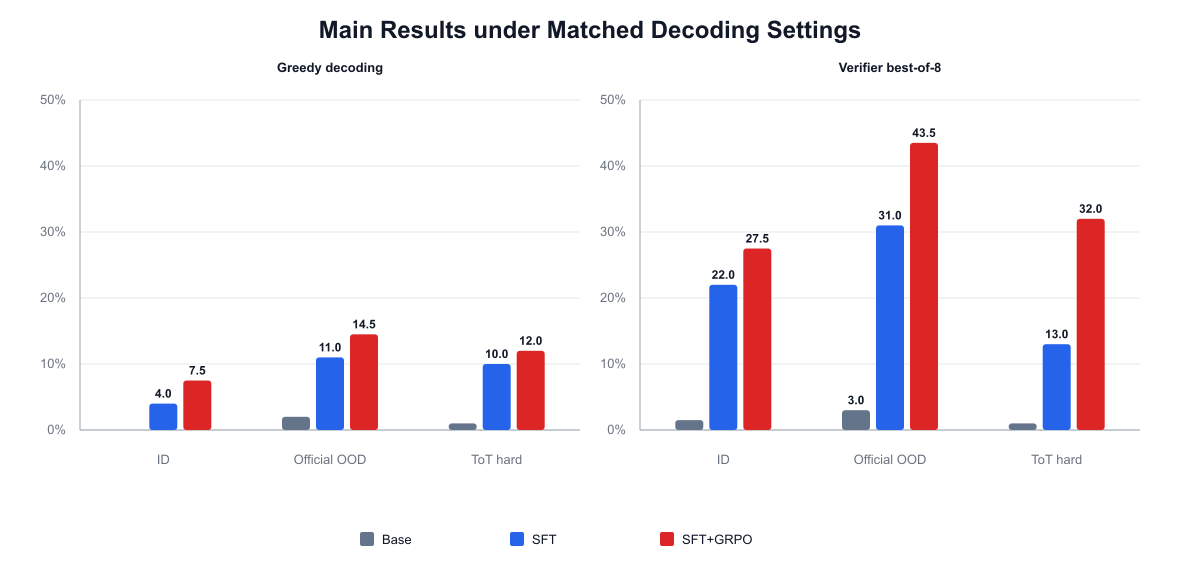
\includegraphics[keepaspectratio,alt={主结果柱状图}]{figures/main_results.png}}
\caption{主结果柱状图}
\end{figure}

基础模型几乎无法稳定完成任务，且不可解样本幻觉率达到 100\%。SFT 后 format rate 达到 100\%，不可解幻觉显著下降，说明 warm-up 解决了格式和拒答基础能力。图中分别在 greedy 与 best-of-8 两种一致解码设置下比较三个训练阶段：GRPO 在 greedy 下提升有限，但在 best-of-8 下显著提升 OOD 和 hard split，说明它主要改善候选池质量。

\subsection{Verifier-based Test-time Compute}\label{verifier-based-test-time-compute-1}

{\def\LTcaptype{none} % do not increment counter
\begin{longtable}[]{@{}lrrrr@{}}
\toprule\noalign{}
解码 & ID & Official OOD & ToT hard & 不可解幻觉 \\
\midrule\noalign{}
\endhead
\bottomrule\noalign{}
\endlastfoot
greedy & 7.5\% & 14.5\% & 12.0\% & 34.0\% \\
best-of-1 & 4.5\% & 10.5\% & 2.0\% & 50.0\% \\
best-of-4 & 15.0\% & 25.5\% & 14.0\% & 7.0\% \\
best-of-8 & 27.5\% & 43.5\% & 32.0\% & 1.0\% \\
best-of-16 & \textbf{44.0\%} & \textbf{65.5\%} & \textbf{49.0\%} & \textbf{0.0\%} \\
\end{longtable}
}

\begin{figure}
\centering
\pandocbounded{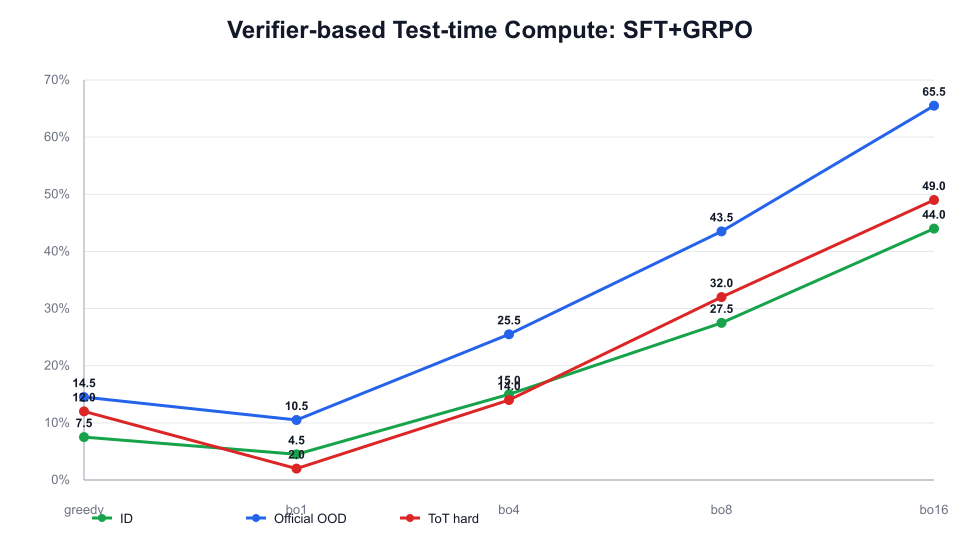
\includegraphics[keepaspectratio,alt={Best-of-N 曲线}]{figures/best_of_sweep.png}}
\caption{Best-of-N 曲线}
\end{figure}

\begin{figure}
\centering
\pandocbounded{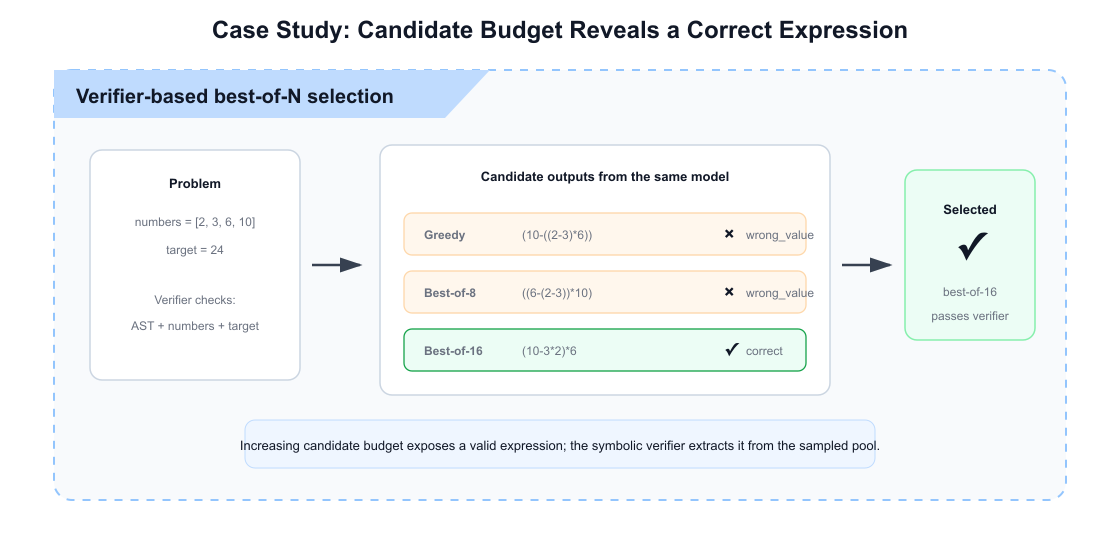
\includegraphics[keepaspectratio,alt={Best-of-N 定性案例}]{figures/case_study_bestof.png}}
\caption{Best-of-N 定性案例}
\end{figure}

以输入 \texttt{{[}2,3,6,10{]}} 为例，greedy 和 best-of-8 记录的候选均因 \texttt{wrong\_value} 未通过验证，而 best-of-16 生成了合法表达式 \texttt{(10-3*2)*6=24}。该案例直观说明：增加候选预算并不改变模型参数，而是提高正确表达式进入候选池的概率，再由符号验证器完成可靠筛选。

best-of-N 是我们本次实验最明显的增益来源。对 \texttt{SFT+GRPO}，Official OOD 从 best-of-1 的 10.5\% 提升到 best-of-16 的 65.5\%，ToT hard 从 2.0\% 提升到 49.0\%。这说明模型单次输出仍不稳定，但候选池中已经包含大量可由 verifier 筛出的正确表达式。

\subsection{不可解样本 Hallucination 分析}\label{ux4e0dux53efux89e3ux6837ux672c-hallucination-ux5206ux6790}

\begin{figure}
\centering
\pandocbounded{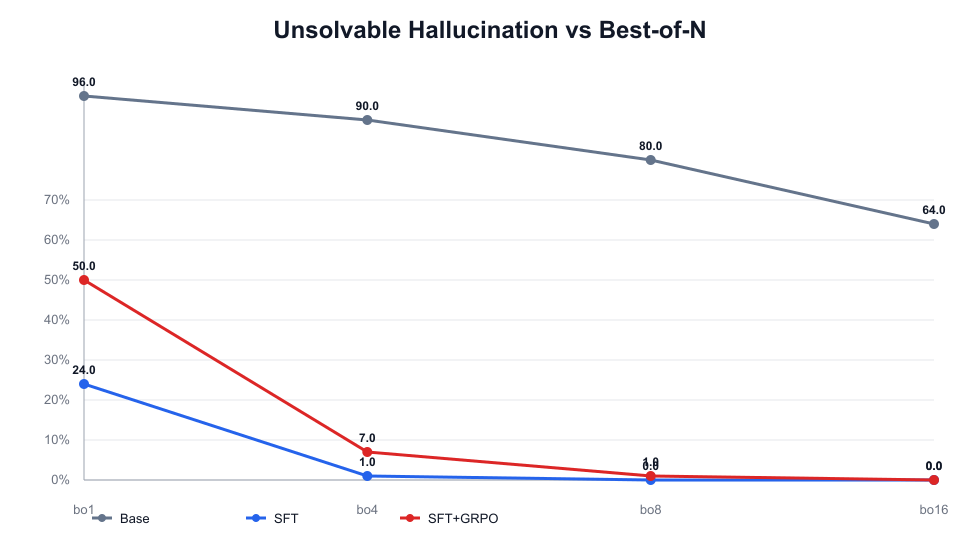
\includegraphics[keepaspectratio,alt={不可解幻觉率}]{figures/hallucination.png}}
\caption{不可解幻觉率}
\end{figure}

不可解样本用于检查模型是否会强行编造答案。Base 在 best-of-1 到 best-of-16 下幻觉率仍高达 96.0\% 到 64.0\%。SFT 显著改善拒答能力，best-of-8 后幻觉率降为 0.0\%。\texttt{SFT+GRPO} 的 greedy 幻觉率升至 34.0\%，说明 RL 更新会扰动拒答行为；但 verifier best-of-16 最终将幻觉率降到 0.0\%。

\subsection{GRPO 训练稳定性与超参对照}\label{grpo-ux8badux7ec3ux7a33ux5b9aux6027ux4e0eux8d85ux53c2ux5bf9ux7167}

{\def\LTcaptype{none} % do not increment counter
\begin{longtable}[]{@{}
  >{\raggedright\arraybackslash}p{(\linewidth - 12\tabcolsep) * \real{0.1111}}
  >{\raggedleft\arraybackslash}p{(\linewidth - 12\tabcolsep) * \real{0.1481}}
  >{\raggedleft\arraybackslash}p{(\linewidth - 12\tabcolsep) * \real{0.1481}}
  >{\raggedleft\arraybackslash}p{(\linewidth - 12\tabcolsep) * \real{0.1481}}
  >{\raggedleft\arraybackslash}p{(\linewidth - 12\tabcolsep) * \real{0.1481}}
  >{\raggedleft\arraybackslash}p{(\linewidth - 12\tabcolsep) * \real{0.1481}}
  >{\raggedleft\arraybackslash}p{(\linewidth - 12\tabcolsep) * \real{0.1481}}@{}}
\toprule\noalign{}
\begin{minipage}[b]{\linewidth}\raggedright
GRPO 配置
\end{minipage} & \begin{minipage}[b]{\linewidth}\raggedleft
Greedy OOD
\end{minipage} & \begin{minipage}[b]{\linewidth}\raggedleft
Greedy hard
\end{minipage} & \begin{minipage}[b]{\linewidth}\raggedleft
Greedy 幻觉
\end{minipage} & \begin{minipage}[b]{\linewidth}\raggedleft
Best-of-8 OOD
\end{minipage} & \begin{minipage}[b]{\linewidth}\raggedleft
Best-of-8 hard
\end{minipage} & \begin{minipage}[b]{\linewidth}\raggedleft
Best-of-8 幻觉
\end{minipage} \\
\midrule\noalign{}
\endhead
\bottomrule\noalign{}
\endlastfoot
\texttt{8e-7/s300/g8} & 14.5\% & 12.0\% & 34.0\% & \textbf{43.5\%} & \textbf{32.0\%} & 1.0\% \\
\texttt{3e-7/s300/g8} & 13.0\% & 11.0\% & \textbf{17.0\%} & 39.0\% & 25.0\% & \textbf{0.0\%} \\
\texttt{3e-7/s600/g8} & \textbf{15.0\%} & 11.0\% & 25.0\% & 41.5\% & 31.0\% & 2.0\% \\
\end{longtable}
}

\begin{figure}
\centering
\pandocbounded{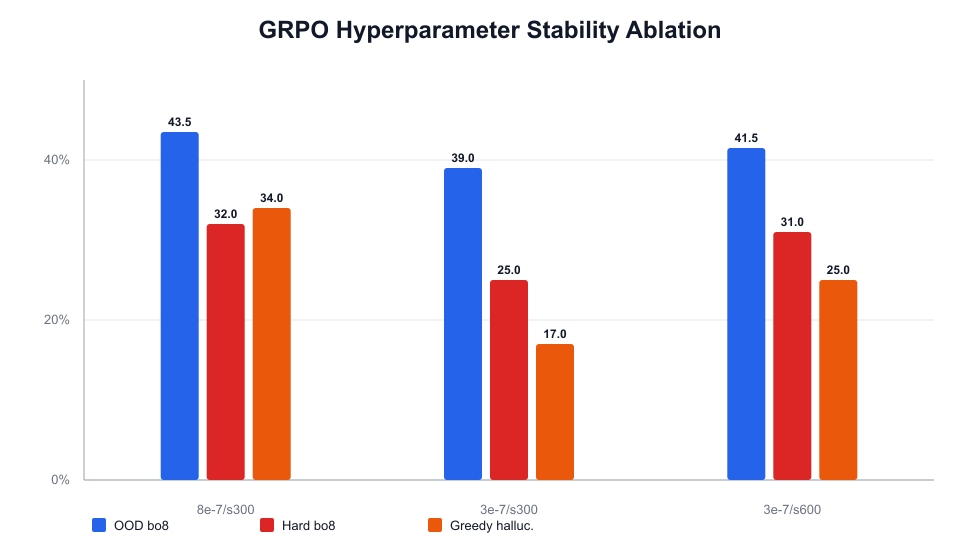
\includegraphics[keepaspectratio,alt={GRPO 超参对照}]{figures/grpo_ablation.png}}
\caption{GRPO 超参对照}
\end{figure}

低学习率能缓解 greedy 下的不可解幻觉，其中 \texttt{3e-7/s300} 将 greedy 幻觉率从 34.0\% 降至 17.0\%。但主线 \texttt{8e-7/s300/g8} 在 best-of-8 的 OOD 与 ToT hard 上仍最强。因此最终采用主线配置作为主要结果，并将低学习率实验作为训练稳定性分析。

\subsection{训练曲线}\label{ux8badux7ec3ux66f2ux7ebf}

\begin{figure}
\centering
\pandocbounded{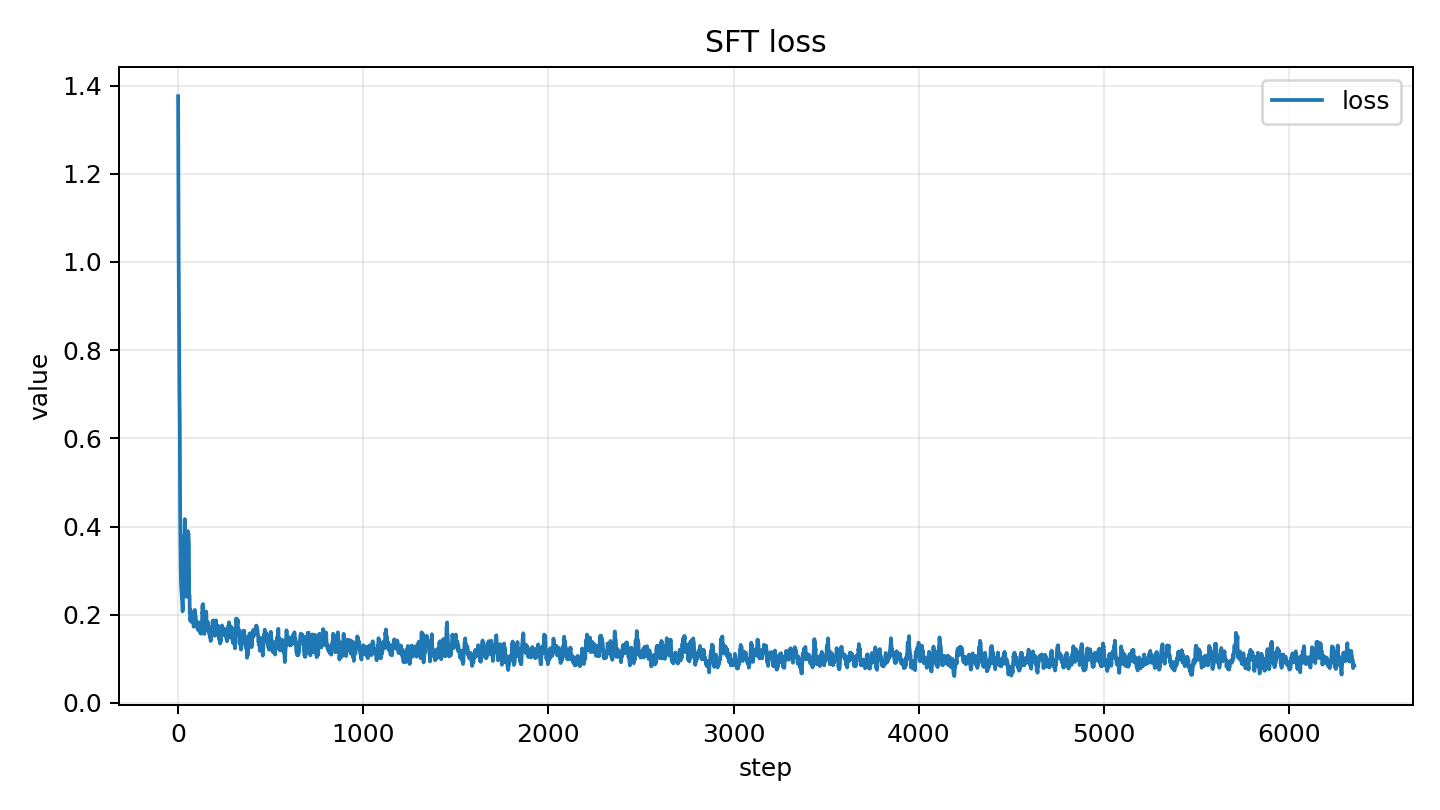
\includegraphics[keepaspectratio,alt={SFT loss}]{figures/sft_loss.png}}
\caption{SFT loss}
\end{figure}

\begin{figure}
\centering
\pandocbounded{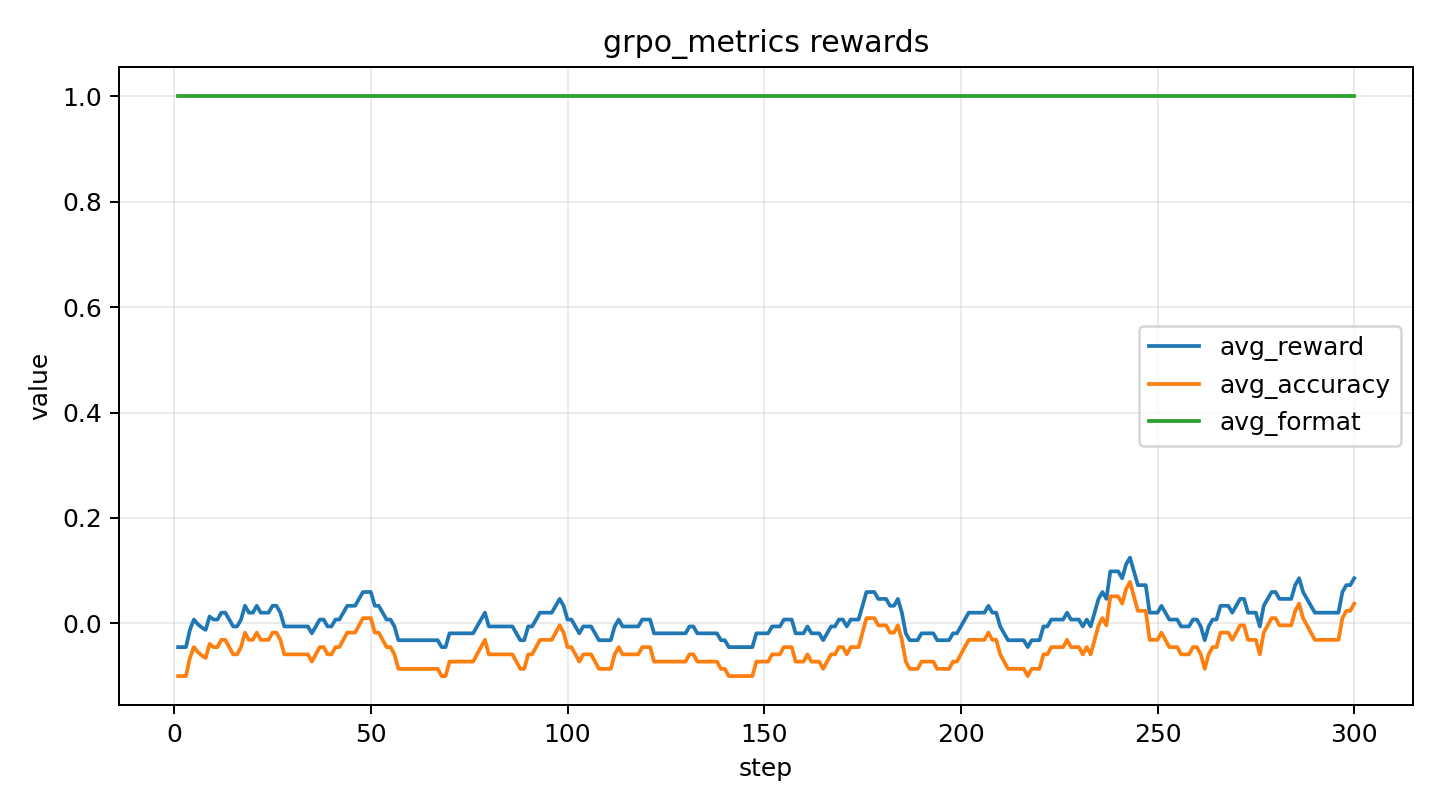
\includegraphics[keepaspectratio,alt={GRPO reward}]{figures/grpo_reward.png}}
\caption{GRPO reward}
\end{figure}

\begin{figure}
\centering
\pandocbounded{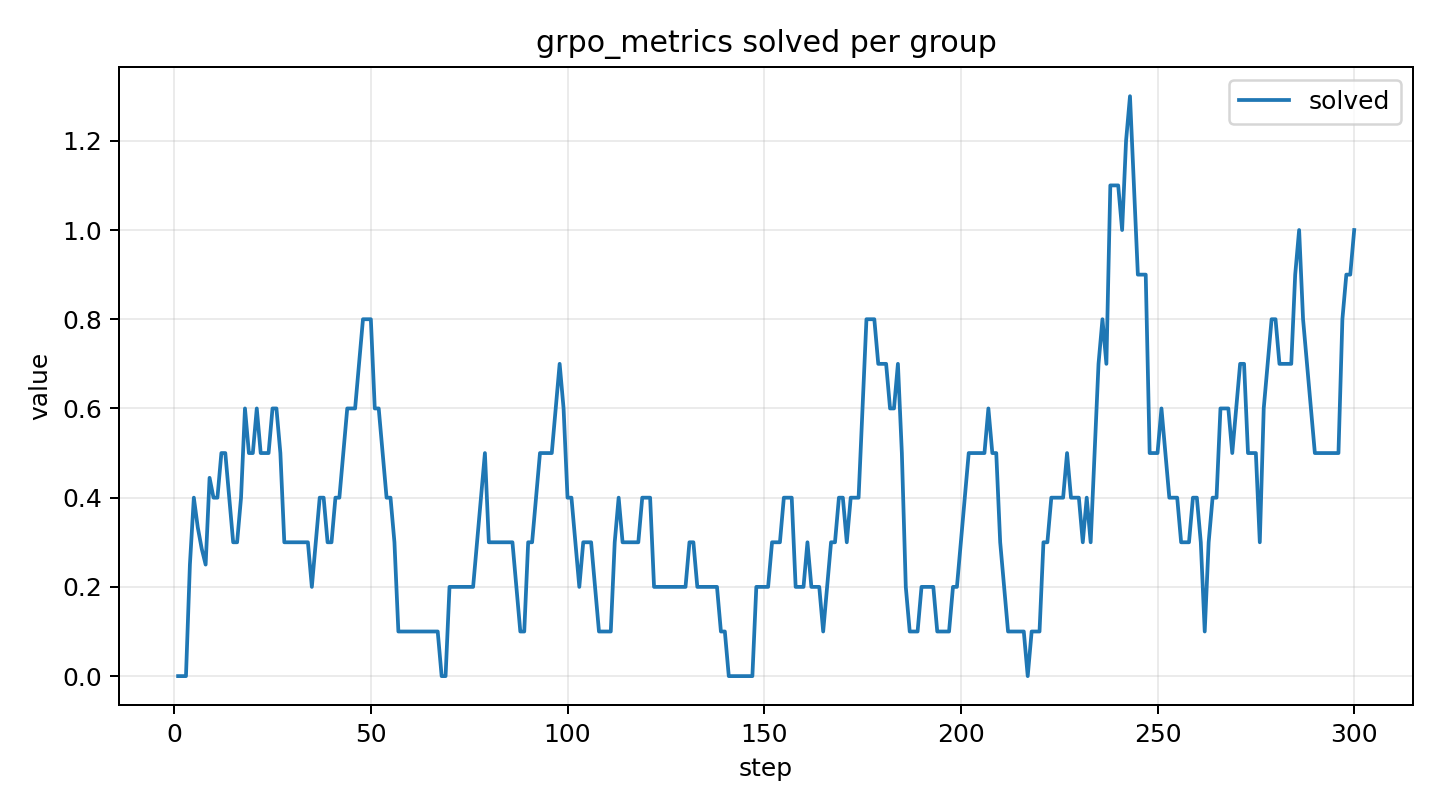
\includegraphics[keepaspectratio,alt={GRPO solved per group}]{figures/grpo_solved.png}}
\caption{GRPO solved per group}
\end{figure}

SFT loss 持续下降，说明 warm-up 阶段稳定学习了输出格式和表达式模式。GRPO 的 reward 与 solved per group 存在波动，符合强化学习训练不稳定的预期。主线 GRPO 最后 50 step 的平均 reward 为 0.0412，平均 solved per group 为 0.66，说明训练后期候选池中正确表达式比例有所增加。

\subsection{错误类型分析}\label{ux9519ux8befux7c7bux578bux5206ux6790}

以最终 \texttt{SFT+GRPO\ +\ best-of-16} 为例，主要错误如下：

{\def\LTcaptype{none} % do not increment counter
\begin{longtable}[]{@{}
  >{\raggedright\arraybackslash}p{(\linewidth - 2\tabcolsep) * \real{0.5000}}
  >{\raggedright\arraybackslash}p{(\linewidth - 2\tabcolsep) * \real{0.5000}}@{}}
\toprule\noalign{}
\begin{minipage}[b]{\linewidth}\raggedright
Split
\end{minipage} & \begin{minipage}[b]{\linewidth}\raggedright
主要错误
\end{minipage} \\
\midrule\noalign{}
\endhead
\bottomrule\noalign{}
\endlastfoot
ID & \texttt{wrong\_value=74}, \texttt{refusal\_or\_no\_answer=38} \\
Official OOD & \texttt{wrong\_value=38}, \texttt{refusal\_or\_no\_answer=31} \\
ToT hard & \texttt{wrong\_value=38}, \texttt{refusal\_or\_no\_answer=12}, \texttt{invalid\_expression=1} \\
Unsolvable & \texttt{refused=100} \\
\end{longtable}
}

\begin{figure}
\centering
\pandocbounded{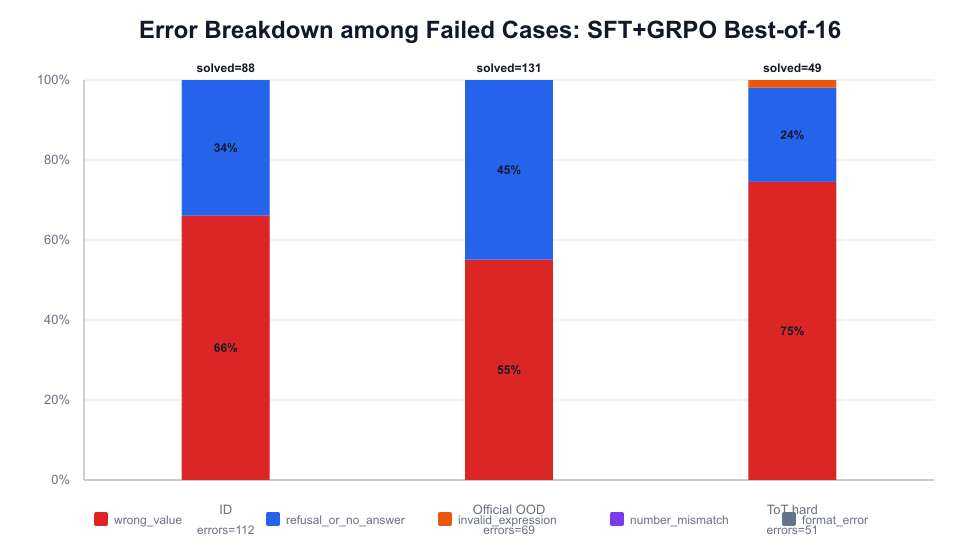
\includegraphics[keepaspectratio,alt={错误类型堆叠图}]{figures/error_breakdown.png}}
\caption{错误类型堆叠图}
\end{figure}

SFT 后格式错误基本消失，最终配置的失败样本主要由 \texttt{wrong\_value} 与 \texttt{refusal\_or\_no\_answer} 构成，其中 ToT hard 的失败样本中约 75\% 为 \texttt{wrong\_value}。这说明瓶颈已经从``格式学习''转向``算术搜索与组合推理''。在不可解 split 上，最终配置 100 个样本全部拒答，说明 verifier-based selection 能有效抑制幻觉。

\subsection{Hard Split 难度分析}\label{hard-split-ux96beux5ea6ux5206ux6790}

{\def\LTcaptype{none} % do not increment counter
\begin{longtable}[]{@{}
  >{\raggedright\arraybackslash}p{(\linewidth - 8\tabcolsep) * \real{0.1579}}
  >{\raggedleft\arraybackslash}p{(\linewidth - 8\tabcolsep) * \real{0.2105}}
  >{\raggedleft\arraybackslash}p{(\linewidth - 8\tabcolsep) * \real{0.2105}}
  >{\raggedleft\arraybackslash}p{(\linewidth - 8\tabcolsep) * \real{0.2105}}
  >{\raggedleft\arraybackslash}p{(\linewidth - 8\tabcolsep) * \real{0.2105}}@{}}
\toprule\noalign{}
\begin{minipage}[b]{\linewidth}\raggedright
Split
\end{minipage} & \begin{minipage}[b]{\linewidth}\raggedleft
样本数
\end{minipage} & \begin{minipage}[b]{\linewidth}\raggedleft
官方平均 solved rate
\end{minipage} & \begin{minipage}[b]{\linewidth}\raggedleft
平均 rank
\end{minipage} & \begin{minipage}[b]{\linewidth}\raggedleft
SFT+GRPO best-of-16
\end{minipage} \\
\midrule\noalign{}
\endhead
\bottomrule\noalign{}
\endlastfoot
Official OOD & 200 & 96.98\% & 100.5 & 65.5\% \\
ToT hard 900-1000 & 100 & 85.88\% & 950.5 & 49.0\% \\
\end{longtable}
}

\begin{figure}
\centering
\pandocbounded{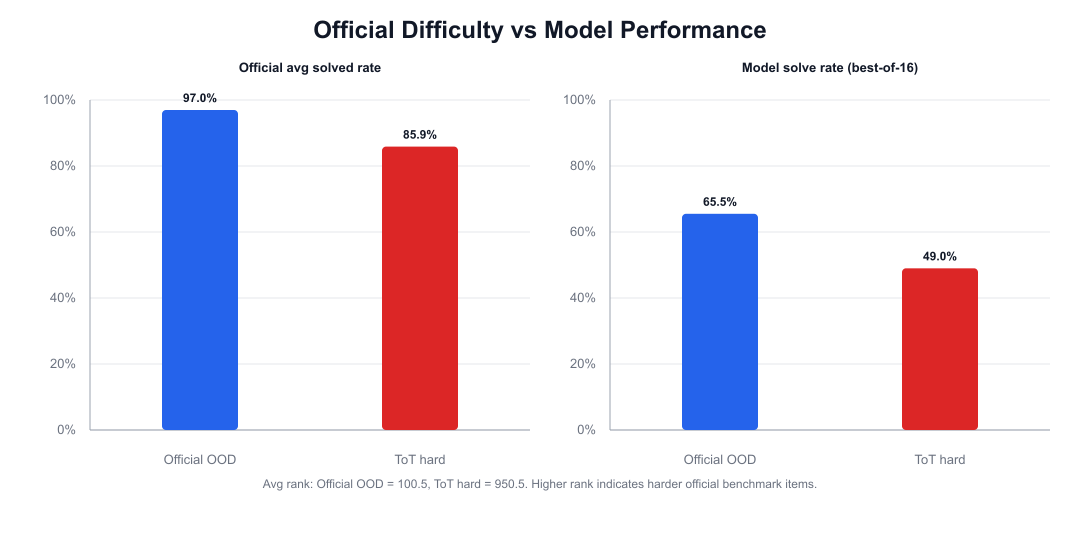
\includegraphics[keepaspectratio,alt={Hard split 难度分析}]{figures/difficulty_analysis.png}}
\caption{Hard split 难度分析}
\end{figure}

ToT hard 来自 official benchmark 的 indices 900-1000，平均 rank 明显更高，官方 solved rate 更低，因此比普通 OOD 更困难。模型在 hard split 上仍达到 49.0\%，说明 verifier best-of-N 不只提升简单题，也能提升困难组合题表现。

\subsection{Countdown 加分项}\label{countdown-ux52a0ux5206ux9879}

Countdown 任务将输入扩展为 3-4 个数字和任意 target，用于验证 target-aware 框架是否可迁移。

{\def\LTcaptype{none} % do not increment counter
\begin{longtable}[]{@{}llrr@{}}
\toprule\noalign{}
模型阶段 & 解码 & Countdown solve & Format \\
\midrule\noalign{}
\endhead
\bottomrule\noalign{}
\endlastfoot
SFT & greedy & 10.5\% & 100.0\% \\
SFT & best-of-8 & \textbf{42.0\%} & 100.0\% \\
SFT+GRPO & greedy & 11.0\% & 100.0\% \\
SFT+GRPO & best-of-8 & 40.5\% & 100.0\% \\
\end{longtable}
}

\begin{figure}
\centering
\pandocbounded{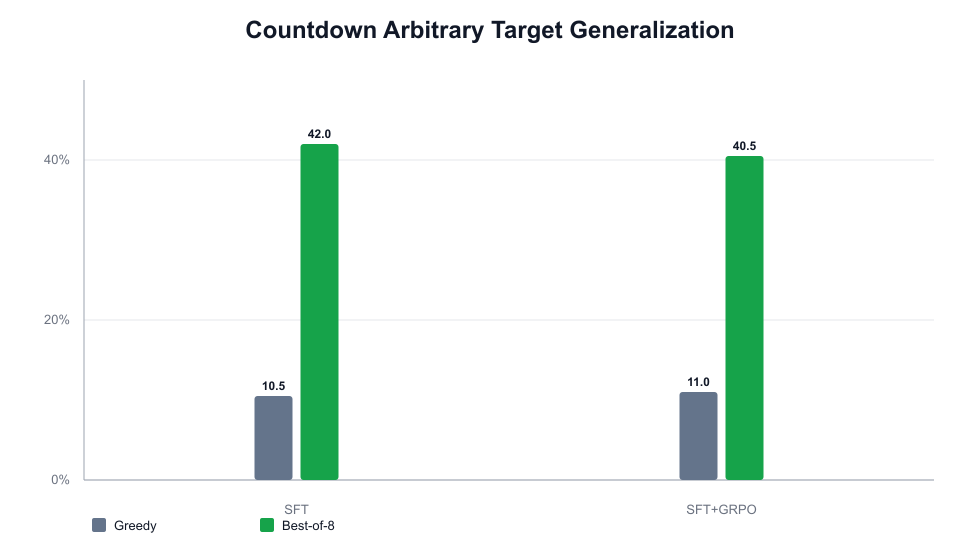
\includegraphics[keepaspectratio,alt={Countdown 结果}]{figures/countdown.png}}
\caption{Countdown 结果}
\end{figure}

Countdown 结果证明同一套 prompt、target-aware verifier 和 reward 可以迁移到任意目标数构造任务。best-of-8 相比 greedy 提升明显，但小规模 Countdown GRPO 未超过 SFT best-of-8，因此该部分更适合作为框架迁移验证，而不是声称 GRPO 在 Countdown 上带来显著增益。

\section{结论}\label{ux7ed3ux8bba}

\subsection{局限性}\label{ux5c40ux9650ux6027}

\begin{enumerate}
\def\labelenumi{\arabic{enumi}.}
\tightlist
\item
  \textbf{Greedy 成功率仍低。} 最终模型 greedy OOD 只有 14.5\%，说明模型尚未稳定内化完整算术搜索策略。
\item
  \textbf{Best-of-N 带来额外推理成本。} best-of-16 显著提升性能，但每题需要采样更多候选。
\item
  \textbf{GRPO 会扰动拒答能力。} 主线 GRPO greedy hallucination 从 SFT 的 4.0\% 升至 34.0\%，需要 verifier 或更保守超参控制。
\item
  \textbf{Countdown GRPO 增益有限。} Countdown 上 SFT best-of-8 为 42.0\%，SFT+GRPO best-of-8 为 40.5\%，说明任意目标任务仍需要更充分训练。
\item
  \textbf{训练规模较小。} 主线 GRPO 只使用 300 prompts，结果更适合作为小规模 RLVR 验证，而非性能上限。
\end{enumerate}

\subsection{总结}\label{ux603bux7ed3}

本次实验我们完成了基于 \texttt{Qwen2.5-1.5B-Instruct} 的 24 点游戏 RLVR 实验。SFT warm-up 解决了基础模型格式不稳和不可解幻觉问题，GRPO 进一步提升了候选池质量，而 verifier-based best-of-N 将 OOD 和 hard split 表现显著放大。最终 \texttt{SFT+GRPO\ +\ best-of-16} 在 Official OOD 上达到 65.5\%，在 ToT hard 上达到 49.0\%，不可解幻觉率为 0.0\%。

从建模角度看，项目不只是复现 GRPO，而是围绕 24 点任务补充了 target-aware 扩展、不可解幻觉评估、test-time verifier selection、错误类型诊断和 hard split 难度分析。这些设计使实验结果更可解释，也更适合作为 RLVR 在小规模可验证推理任务上的完整案例。

\section{参考文献}\label{ux53c2ux8003ux6587ux732e}

\small
\sloppy

\begin{enumerate}
\def\labelenumi{\arabic{enumi}.}
\tightlist
\item
  Shao Z, Wang P, Zhu Q, et al.~DeepSeekMath: Pushing the Limits of Mathematical Reasoning in Open Language Models{[}EB/OL{]}. arXiv:2402.03300, 2024. \url{https://arxiv.org/abs/2402.03300}.
\item
  DeepSeek-AI, Guo D, Yang D, et al.~DeepSeek-R1: Incentivizing Reasoning Capability in LLMs via Reinforcement Learning{[}EB/OL{]}. arXiv:2501.12948, 2025. \url{https://arxiv.org/abs/2501.12948}.
\item
  Yang A, Yang B, Zhang B, et al.~Qwen2.5 Technical Report{[}EB/OL{]}. arXiv:2412.15115, 2024. \url{https://arxiv.org/abs/2412.15115}.
\item
  Qwen Team. Qwen2.5-1.5B-Instruct Model Card{[}EB/OL{]}. Hugging Face, 2024. \url{https://huggingface.co/Qwen/Qwen2.5-1.5B-Instruct}.
\item
  Yao S, Yu D, Zhao J, et al.~Tree of Thoughts: Deliberate Problem Solving with Large Language Models{[}C{]}//Advances in Neural Information Processing Systems. 2023. \url{https://arxiv.org/abs/2305.10601}.
\item
  Pan J, et al.~TinyZero: Minimal Reproduction of DeepSeek R1-Zero{[}EB/OL{]}. GitHub, 2025. \url{https://github.com/Jiayi-Pan/TinyZero}.
\item
  Xie T, Gao Z, Ren Q, et al.~Logic-RL: Unleashing LLM Reasoning with Rule-Based Reinforcement Learning{[}EB/OL{]}. arXiv:2502.14768, 2025. \url{https://arxiv.org/abs/2502.14768}.
\item
  Hu E J, Shen Y, Wallis P, et al.~LoRA: Low-Rank Adaptation of Large Language Models{[}C{]}//International Conference on Learning Representations. 2022. \url{https://arxiv.org/abs/2106.09685}.
\item
  Hugging Face. TRL GRPO Trainer Documentation{[}EB/OL{]}. \url{https://huggingface.co/docs/trl/en/grpo_trainer}.
\item
  Hugging Face. Open-R1: A Fully Open Reproduction of DeepSeek-R1{[}EB/OL{]}. GitHub, 2025. \url{https://github.com/huggingface/open-r1}.
\item
  nlile. 24-game Dataset{[}DB/OL{]}. Hugging Face. \url{https://huggingface.co/datasets/nlile/24-game}.
\item
  test-time-compute. Game-of-24 Dataset{[}DB/OL{]}. Hugging Face. \url{https://huggingface.co/datasets/test-time-compute/game-of-24}.
\item
  Pan J. Countdown-Tasks-3to4 Dataset{[}DB/OL{]}. Hugging Face. \url{https://huggingface.co/datasets/Jiayi-Pan/Countdown-Tasks-3to4}.
\end{enumerate}

\normalsize
\fussy

\section{附录：复现命令与结果路径}\label{ux9644ux5f55ux590dux73b0ux547dux4ee4ux4e0eux7ed3ux679cux8defux5f84}

\subsection{主线实验}\label{ux4e3bux7ebfux5b9eux9a8c}

\begin{Shaded}
\begin{Highlighting}[]
\BuiltInTok{export} \VariableTok{PYTHONPATH}\OperatorTok{=}\VariableTok{$PWD}
\BuiltInTok{export} \VariableTok{QWEN\_15B}\OperatorTok{=}\NormalTok{/path/to/Qwen2.5{-}1.5B{-}Instruct}

\BuiltInTok{export} \VariableTok{N\_EVAL}\OperatorTok{=}\NormalTok{200}
\BuiltInTok{export} \VariableTok{N\_HARD}\OperatorTok{=}\NormalTok{100}
\BuiltInTok{export} \VariableTok{BEST\_OF}\OperatorTok{=}\NormalTok{8}
\BuiltInTok{export} \VariableTok{GRPO\_SAMPLES}\OperatorTok{=}\NormalTok{300}
\BuiltInTok{export} \VariableTok{GRPO\_GENERATIONS}\OperatorTok{=}\NormalTok{8}
\FunctionTok{bash}\NormalTok{ scripts/run\_15b\_mainline.sh }\StringTok{"}\VariableTok{$QWEN\_15B}\StringTok{"}\NormalTok{ 0}
\end{Highlighting}
\end{Shaded}

\subsection{Best-of-N Sweep}\label{best-of-n-sweep}

\begin{Shaded}
\begin{Highlighting}[]
\BuiltInTok{export} \VariableTok{N\_EVAL}\OperatorTok{=}\NormalTok{200}
\BuiltInTok{export} \VariableTok{N\_HARD}\OperatorTok{=}\NormalTok{100}
\BuiltInTok{export} \VariableTok{BEST\_OF\_LIST}\OperatorTok{=}\StringTok{"1 4 8 16"}
\FunctionTok{bash}\NormalTok{ scripts/run\_ttc\_sweep.sh }\StringTok{"}\VariableTok{$QWEN\_15B}\StringTok{"}\NormalTok{ 0}
\end{Highlighting}
\end{Shaded}

\subsection{Countdown 加分项}\label{countdown-ux52a0ux5206ux9879-1}

\begin{Shaded}
\begin{Highlighting}[]
\BuiltInTok{export} \VariableTok{COUNTDOWN\_TRAIN}\OperatorTok{=}\NormalTok{3000}
\BuiltInTok{export} \VariableTok{COUNTDOWN\_EVAL}\OperatorTok{=}\NormalTok{200}
\BuiltInTok{export} \VariableTok{BEST\_OF}\OperatorTok{=}\NormalTok{8}
\BuiltInTok{export} \VariableTok{GRPO\_SAMPLES}\OperatorTok{=}\NormalTok{300}
\BuiltInTok{export} \VariableTok{GRPO\_GENERATIONS}\OperatorTok{=}\NormalTok{8}
\FunctionTok{bash}\NormalTok{ scripts/run\_countdown\_bonus.sh }\StringTok{"}\VariableTok{$QWEN\_15B}\StringTok{"}\NormalTok{ 0}
\end{Highlighting}
\end{Shaded}

\subsection{关键结果路径}\label{ux5173ux952eux7ed3ux679cux8defux5f84}

{\def\LTcaptype{none} % do not increment counter
\begin{longtable}[]{@{}
  >{\raggedright\arraybackslash}p{(\linewidth - 2\tabcolsep) * \real{0.5000}}
  >{\raggedright\arraybackslash}p{(\linewidth - 2\tabcolsep) * \real{0.5000}}@{}}
\toprule\noalign{}
\begin{minipage}[b]{\linewidth}\raggedright
内容
\end{minipage} & \begin{minipage}[b]{\linewidth}\raggedright
路径
\end{minipage} \\
\midrule\noalign{}
\endhead
\bottomrule\noalign{}
\endlastfoot
1.5B base 评估 & \texttt{results/game24-15b-base/} \\
1.5B SFT 评估与曲线 & \texttt{results/game24-sft-15b-curriculum/} \\
1.5B SFT+GRPO 评估与曲线 & \texttt{results/game24-grpo-15b-curriculum/} \\
GRPO 超参对照 & \texttt{results/game24-grpo-15b-lr3e-7-s300/}, \texttt{results/game24-grpo-15b-lr3e-7-s600/} \\
Countdown 加分项 & \texttt{results/countdown-sft-15b/}, \texttt{results/countdown-grpo-15b/} \\
报告图表 & \texttt{docs/report/figures/} \\
\end{longtable}
}

早期 0.5B direct GRPO 和 3B 预实验保留在 \texttt{results/} 中作为探索过程归档。由于训练协议不同，它们不作为正式模型规模对照。

\end{document}
